\section{Experimental Evaluation of \ac{UV} \ac{AMBC} \\
            with Unmodeled Actuator Dynamics}
\label{chUV_AMBC.sec.unmodeledActDyn}



%As discussed in the introduction to Section
%\ref{chUV_AMBC.sec.theory}, the widespread realization of tracking
%performance gains provided by \ac{UV} \ac{MBC} might require \ac{AMBC}
%since \ac{UV} mass and drag parameters can not be computed
%analytically.
%TM_ADD_IN_IDEA? The introduction to Chapter \ref{chUV_AID} talks more
%about the inability to analytically commpute parameters... 
%
This Section reports a comparative experimental evaluation between
\ac{UV} \ac{AMBC} and \ac{UV} \ac{PDC} for typical operational
maneuvers.
%
Although experimental implementations of \ac{UV} \ac{AMBC} algorithms
have been reported\cite{yoerger.icra91, yuhICRA1999,
  antonelli&sarkar.cst2001, smallwood2004JOE, maalouf2013pd,
  zhao2005experimental}, to the best of our knowledge experimental
evaluations of \ac{AMBC} during simultaneous motion in all \ac{DOF}
has not previously been reported.
%
The comparative experimental evaluation of \ac{AMBC} and \ac{PDC}
during simultaneous 6-\ac{DOF} maneuvers reported herein shows that
\ac{AMBC} can provide better position tracking performance than
\ac{PDC}.


This Section is organized as follows:
%
%Section \ref{chUV_AMBC.sec.twoStepMethod} reports a two-step \ac{AMBC}
%algorithm shown experimentally to be robust to actuator modeling
%errors observed in our experimental vehicle.
%
Section \ref{chUV_AMBC.sec.fullAnalysisFailure} shows how direct
implementation of the \ac{AMBC} from Theorem
\ref{chUV_AMBC.theo.UV_AMBC} exhibits unstable parameter adaptation
in the presence of unmodeled thrust reversal dynamics.
%
Section \ref{chUV_AMBC.sec.singleDOFAnalysisFailure} presents two
experiments where \ac{AMBC} is used to follow a pitch-only reference
trajectory.
%
The range of motion is changed such that one pitch-only reference
trajectory requires thrust reversals and the other pitch-only
reference trajectory does not.
%
A comparative analysis of these parameter adaption processes details
how unmodeled dynamics arising from thrust reversals can cause
unstable parameter adaptation.
%
Finally, Section \ref{chUV_AMBC.sec.twoStepExp} reports an
experimental evaluation of the two-step \ac{AMBC} algorithm reported
in Section \ref{chUV_AMBC.sec.twoStepMethod}, and an experimental
comparison of two-step \ac{AMBC} and \ac{PDC}.



\subsection{Experimental Setup}
\label{chUV_AMBC.sec.expSetup}


We employed the Johns Hopkins University Hydrodynamic Test Facility
(Appendix \ref{appenJHUHTF}) to evaluate \ac{UV} \ac{AMBC}.
%
To compare the trajectory-tracking performance of controllers we
consider the \ac{MNE} for vectors such as the position error ($\Delta
\psi$) and velocity error ($\Delta v$).
%
We also report the \ac{MAE} between the measured and reference
values for the 12 position and velocity signals.
%
A smaller \ac{MNE} or \ac{MAE} value means the controller is doing a
better job tracking the reference trajectory.
%
As with the adaptively identified \ac{UV} models in Sections
\ref{chUV_AID.sec.UVSO3exp} and \ref{chUV_AID.sec.UVSE3exp},
identified \ac{UV} models are evaluated by error between simulated
model performance and the experimentally observed performance.
%
\ac{MAE} values between the simulated plant states and
experimentally measured states are reported.
%
Appendix \ref{appenJHUHTF} provides further details about
our hydrodynamic test facility and algorithm evaluation methods.


The fully-coupled model of \ac{UV} dynamics used in
(\ref{chUV_AMBC.eq.UVSE3plant}) requires 241 independent parameter
values.
%
To simplify and clarify the experimental analysis of \ac{UV} \ac{AMBC}
in the presence of unmodeled thruster dynamics, we have implemented a
controller which employs an uncoupled model using 16 scalar terms: 6
hydrodynamic mass, 6 quadratic drag terms (one for each \ac{DOF} which
we will label as $m_i$ and $d_i$ respectively), and the 4
gravitational parameters $g$ and $b$.
%
For a diagonal parameter adaptation gain matrix $K_\theta$, we can
label the individual mass parameter gains as $\gamma_{m_i}$, the
individual drag parameter gains as $\gamma_{d_i}$, the individual
buoyancy parameter gains as $\gamma_{b_i}$ and the gravitational
parameter gain as $\gamma_{g}$.
%
Both the \ac{AMBC} control process and parameter update process
where implemented as a discrete time approximation of the
continuous time algorithm.
%
Every 100ms the commanded torque and commanded force were recalculated
using (\ref{chUV_AMBC.eq.AMBC_controlLaw}) as well as the most recent
state measurements, reference state values, and parameter estimates.
%
These inputs signals are therefore piecewise constant.
%
Euler integration of (\ref{chUV_AMBC.eq.AMBC_paramUpdateLaw}) for
100ms time steps provided the time series of parameter estimates.
%
The 100ms \ac{JHUROV} control system cycle period is one to two
orders-of-magnitude smaller than the \ac{JHUROV} state variation rate
of 1 second or greater observed during dynamic operation.
%
In practice the discrete time approximations were seen to provide
similar performance to the continuous time algorithm implemented in
simulation.


Sinusoidal reference trajectories are used in this
study. 
%
Table \ref{chUV_AMBC.tb.expStat} lists the frequencies and amplitudes
for the 6-\ac{DOF} reference trajectories used.  


\begin{table}[htbp]
\ssp
\caption{Reference Trajectory Information}
\begin{center}
\begin{tabular}{cccc}
 & & RefTraj1& RefTraj2 \\
\hline
\multicolumn{2}{c}{Reference Trajectory}  &Trajectory Control      &  Parameter \\
\multicolumn{2}{c}{Purpose}              & Evaluation &  Cross-Validation \\
\hline
\ac{DOF}      & {\it Excitation} & \multicolumn{2}{c}{\it Trajectory-Tracking} \\
world x  &  Cos Freq  & 0.242 rad/sec & 0.185 rad/sec \\ 
         &  Cos Amp  &    0.50 m     &     0.50 m    \\ 
\hline
\ac{DOF}      & {\it Excitation} & \multicolumn{2}{c}{\it Trajectory-Tracking} \\
world y  &  Cos Freq  & 0.210 rad/sec & 0.286 rad/sec \\ 
         &  Cos Amp  &    0.50 m     &     0.50 m    \\ 
\hline
\ac{DOF}      & {\it Excitation} & \multicolumn{2}{c}{\it Trajectory-Tracking} \\
world z  &  Cos Freq  & 0.185 rad/sec & 0.242 rad/sec \\ 
         &  Cos Amp  &    0.30 m     &     0.30 m    \\ 
\hline
\ac{DOF}      & {\it Excitation} & {\it Trajectory-Tracking} & {\it Torque Input} \\
roll     &  Cos Frequency  & 0.5 rad/sec & 0.55 rad/sec \\ 
         &  Cos Amplitude  &    6.9$^\circ$    &     35 N m     \\ 
\hline
\ac{DOF}      & {\it Excitation} & {\it Trajectory-Tracking} & {\it Torque Input} \\
pitch    &  Cos Freq  & 0.6 rad/sec & 0.65 rad/sec \\ 
         &  Cos Amp  &    8.6$^\circ$    &     30 N m     \\ 
\hline
\ac{DOF}      & {\it Excitation} & \multicolumn{2}{c}{\it Trajectory-Tracking} \\
heading  &  Cos Freq  & 0.210 rad/sec & 0.0824 rad/sec \\ 
         &  Cos Amp  &    135$^\circ$  &   135$^\circ$   \\  
\hline \end{tabular}
\end{center}
\label{chUV_AMBC.tb.expStat}
%\vspace*{-5mm}
\end{table}

\subsection{\ac{UV} \ac{AMBC} Instability During 6-\ac{DOF} Motion}
\label{chUV_AMBC.sec.fullAnalysisFailure}



This Section reports an experimental evaluation of \ac{AMBC} during
simultaneous motion in all \ac{DOF} which results in unstable parameter
adaptation.
%
%
%Two experiments reveal parameter
%adaptation instability in the presence of unmodeled thruster dynamics
%during thrust reversals. A third experiment does not have thrust
%reversals and parameter estimates remain stable. 
%
In the experiment the mass, drag, and gravitational terms were
initialized to parameters previously identified to model vehicle
performance (tabulated in Tables \ref{chUV_AMBC.tb.quasistatic} and
\ref{chUV_AMBC.tb.dynParam}). The reference trajectory specified was
RefTraj1 from Table \ref{chUV_AMBC.tb.expStat}. The gains used
were $k_p=300$, $k_d=100$ $\gamma_{m_i}=1000$, $\gamma_{d_i}=5000$,
$\gamma_{g}=\gamma_{b_1}=\gamma_{b_2}=0.5$ and $\gamma_{b_3}=10.0$.


Tables \ref{chUV_AMBC.tb.startCloseGrav} and
\ref{chUV_AMBC.tb.startCloseDyn} tabulate the initial and final
parameters identified.  Over this two-hour duration experiment most
parameter values oscillated near their previously identified values,
however $\hat{b}_3(t)$, $\hat{m}_4(t)$, and $\hat{m}_5(t)$ adapted away
from their previously identified values.  As seen in Figure
\ref{chUV_AMBC.fig.m4_m5_Full_Param_Est}, these mass estimates adapt
to physically unrealistic negative values and show no signs of
asymptotic behavior.  
%
The instability observed in this experiment motivated us to examine
the role of unmodeled thruster dynamics in the $\hat{m}_4(t)$ and
$\hat{m}_5(t)$ adaptation process.


\begin{table}[htbp]
\ssp
\caption{Gravitational Parameters Identified During Unstable Parameter Adaptation}
\begin{center}
\begin{tabular}{c|cccc}
      & $g$ & $b_1$ & $b_2$ & $b_3$   \\
      & {\it N} & {\it N m} & {\it N m} & {\it N m} \\ \hline
Init &  3.63 & 1.017 & 3.02 & 300   \\
Final&  -5.71   &  2.6      & 3.53     & 261 \\ 
\end{tabular}
\end{center}
\label{chUV_AMBC.tb.startCloseGrav}
\vspace*{-5mm}
\end{table}


\begin{table}[htbp]
\ssp
\caption{Mass and Drag Parameters Identified During Unstable Parameter Adaptation}
\begin{center}
\begin{tabular}{c|cccc}
 & $m_i(t_o)$ & $m_i(t_f)$ & $d_i(t_o)$ & $d_i(t_f)$ \\ \hline
Trans X \ac{DOF} & 583 {\it kg} & 583 {\it kg}& -1245 {\it $\frac{\text{N}~\text{s}^2}{\text{m}^2}$}& -1005 {\it $\frac{\text{N}~\text{s}^2}{\text{m}^2}$}\\
Trans Y \ac{DOF} & 873 {\it kg} & 769 {\it kg}& -1426 {\it $\frac{\text{N}~\text{s}^2}{\text{m}^2}$}& -1400 {\it $\frac{\text{N}~\text{s}^2}{\text{m}^2}$}\\
Trans Z \ac{DOF} & 1021 {\it kg} & 1031 {\it kg}& -3060 {\it $\frac{\text{N}~\text{s}^2}{\text{m}^2}$}& -3039 {\it $\frac{\text{N}~\text{s}^2}{\text{m}^2}$}\\
Angular X \ac{DOF} & 103.5 {\it kg $\text{m}^2$} & -1.348 {\it kg $\text{m}^2$} & -728.4 {\it N $\text{s}^2$}& -761.5  {\it N $\text{s}^2$}\\
Angular Y \ac{DOF} & 137.1 {\it kg $\text{m}^2$} & 42.5 {\it kg $\text{m}^2$} & -769.1  {\it N $\text{s}^2$}& -681.4  {\it N $\text{s}^2$}\\
Angular Z \ac{DOF} & 106.4 {\it kg $\text{m}^2$} & 41 {\it kg $\text{m}^2$} & -376.2  {\it N $\text{s}^2$}& -393.3  {\it N $\text{s}^2$}\\
\end{tabular}
\end{center}
\label{chUV_AMBC.tb.startCloseDyn}
\vspace*{-5mm}
\end{table}


\begin{center}
\begin{figure}[htbp]
  \begin{center}
    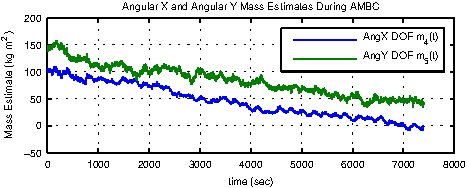
\includegraphics[width=150mm]{./chUV_AMBC/images/m4_m5_Full_Param_EstSm}
  \end{center}
  \caption{ The time evolution of Angular X \ac{DOF} and Angular Y
    \ac{DOF} mass estimates from \ac{AMBC} during 6-\ac{DOF} dynamic
    maneuvers. These mass estimates adapt to physically unrealistic
    negative values and show no signs of asymptotic behavior.}
  \label{chUV_AMBC.fig.m4_m5_Full_Param_Est}
\vspace*{-5mm}
\end{figure}
\end{center}

%\subsection{Background and Paper Contribution}

% In addition to quantifying expected performance gains, it is also
% important that experimental evaluations highlight any unfounded
% assumptions made during the controller's formulation.
% %
% As is shown in Section \ref{sec.fullAnalysisFailure}, the assumption
% that pitch and roll torque applied was close enough to torque
% commanded was not a justified assumption.
% %
% Like the \ac{JHUROV}, many vehicles currently deployed in the open ocean
% are equipped with actuators which can not guarantee the exact force
% commanded will be applied in all operating conditions.
% %
% \ac{UV} \acp{AMBC} have yet to achieve widespread use due to their perceived
% fragility in real world operating conditions.
% %
% We anticipate that this thrust reversal modeling error is one of
% several \ac{UV} \ac{AMBC} failure modes which contribute to this perception.
% %
% However, documenting one such failure mode in laboratory conditions,
% and presenting a modification to \ac{AMBC} which is robust to the
% underlying cause of failure, is an important step to developing \ac{AMBC}
% algorithms which are ready for the open ocean.



%\ac{UV} \acp{AMBC} have yet to achieve widespread use due to their perceived
%fragility in real world operating conditions.
%%
%The \ac{JHUROV}, like many vehicles currently deployed in the open ocean, 
%is equipped with actuators which can not guarantee the exact force
%commanded will be applied in all operating conditions.
%%
%In Section \ref{sec.fullAnalysisFailure} we investigate how modeling
%inaccuracies near thrust reversals can cause unstable parameter
%adaptation.
%%
%We anticipate that this thrust reversal modeling error is one of
%several \ac{UV} \ac{AMBC} failure modes which contribute to the perception of 
%\ac{AMBC} fragility.  
%%
%\hide{We feel documenting this failure mode in laboratory conditions,
%and presenting a modification to \ac{AMBC} which is robust to the
%underlying cause of failure, is an important step to developing \ac{AMBC}
%algorithms which are ready for the open ocean.}


\subsection{Unmodeled Thruster Dynamics within \\
                the \acs{UV} Control Process}

The \ac{JHUROV} control system uses the common assumption of {\it
steady-state} thruster operation when calculating the actuator
commands (see Appendix \ref{appenJHUHTF.sec.hydrolab}).
%
In {\it steady-state} operation at zero advance velocity the axial
thrust of a bladed-propeller marine thruster is linearly proportional
to the applied shaft torque, and is also linearly proportional to the
signed-square of the shaft angular-velocity
\cite{pona.book}.  
%
The parameters of these steady-state thruster models
cannot be determined analytically, but are easily estimated with
simple steady-state experiments.
%
Research has shown that the {\it transient} performance of marine
thrusters can be accurately approximated by a finite-dimensional
second-order plant model of propeller-fluid interaction.
%
The plant parameters of these dynamic thruster models cannot be
determined analytically, and are difficult to estimate experimentally
because such identification requires highly instrumented measurements
of the thruster thrust, prop angular velocity, and fluid flow velocity
in unsteady operation
\cite{yoerger.oe90,healey.joe95,bachmayer&whitcomb&grosenbaugh.joe2000,kim2006accurate}.


Because unsteady thruster model parameters are difficult to obtain
experimentally, in the design of marine vehicle control systems it is
common practice to employ easily-obtained steady-state thruster models.
%
This approach works extremely well for steady-state or slowly
time-varying vehicle motion, but results in the presence of unmodeled 
thruster dynamics during highly dynamic vehicle maneuvering.
%
In 1984, Rohrs et al. famously showed that stable adaptive controllers
for linear time-invariant plants can be destabilized by the presence
of unmodeled plant dynamics \cite{rohrs.1984}. % ,middleton1988design} 
%
To the best of our knowledge, this is the first observation of
unmodeled thruster dynamics resulting in the destabilization of
\ac{AMBC}. %model-based adaptive tracking control of an \ac{UV}.

\subsection{Comparative Experimental Evaluation of \ac{AMBC} \\
                 During Pitch-Only Motion in the Presence \\
                 of Unmodeled Thruster Dynamics}
\label{chUV_AMBC.sec.singleDOFAnalysisFailure}


This Section reports two experiments using \ac{AMBC} to control the
\ac{JHUROV}. In the first experiment parameter adaptation is unstable;
in the second experiment parameter adaptation is stable. In both
experiments the vehicle follows a pitch-only reference trajectory; the
mass, drag, and gravitational terms were initialized to parameters
previously identified to model vehicle performance (tabulated in
Tables \ref{chUV_AMBC.tb.quasistatic} and
\ref{chUV_AMBC.tb.dynParam}); and the gains used were $k_p=300$,
$k_d=100$ $\gamma_{m_i}=1000$, $\gamma_{d_i}=5000$,
$\gamma_{g}=\gamma_{b_1}=\gamma_{b_2}=0.5$ and $\gamma_{b_3}=10.0$.
In the first experiment, the pitch-only reference trajectory
oscillates about zero pitch.  In the second experiment, pitch-only
reference trajectory oscillates about a mean pitch of $5^\circ$ with
an amplitude of $3^\circ$.  The first experiment requires thrust
reversals to follow the specified reference trajectory, and the second
experiment does not require thrust reversals.

Figure \ref{chUV_AMBC.fig.stictionErrorWithThRev} plots the pitch,
angular velocity, thrust commands, and mass estimate derivative for
the experiment with thrust reversals.  In the thrust subplots the four
lines are plotted, the commanded and estimated thrusts are shown for
the two thrusters actuating vehicle pitch.  Note that the thrust is
estimated using a thruster's measured angular velocity as detailed in
Appendix \ref{appenJHUHTF.sec.hydrolab}.  Note that for both thrusters
as the commanded thrust crosses zero, the measured output remains zero
until the commanded thrust reaches 5 Newtons.  The buoyancy torque's
influence causes the pitch and y angular velocity to significantly
deviate from their respective reference trajectories.  From the
perspective of the \ac{AMBC} algorithm, these deviations from the
position and velocity reference trajectories are indistinguishable
from the deviations which would occur if the estimated pitch inertia
were too large, thus the parameter estimate update for this term,
$\dot{\hat{m}}_5$, has a large negative spike after each thrust
reversal. Over a multi-hour experiment this systematic error causes
pitch and roll mass estimates to adapt to physically unrealistic
negative values.

Figure \ref{chUV_AMBC.fig.stictionErrorWithoutThRev} plots the pitch,
angular velocity, thrust commands, and mass estimate derivative for
the experiment without thrust reversals.  Without thrust reversals,
the chain of events leading to a large negative spike in the pitch
mass update law are not present. The balanced parameter adaptation
seen in this third experiment leads to pitch mass convergence to a
physically realistic value.

%The conditions for this type of ___ also exist in the roll DOF, but not
%in the other DOF of x, y, z, Heading

\begin{center}
\begin{figure*}[htbp]
  \begin{center}
    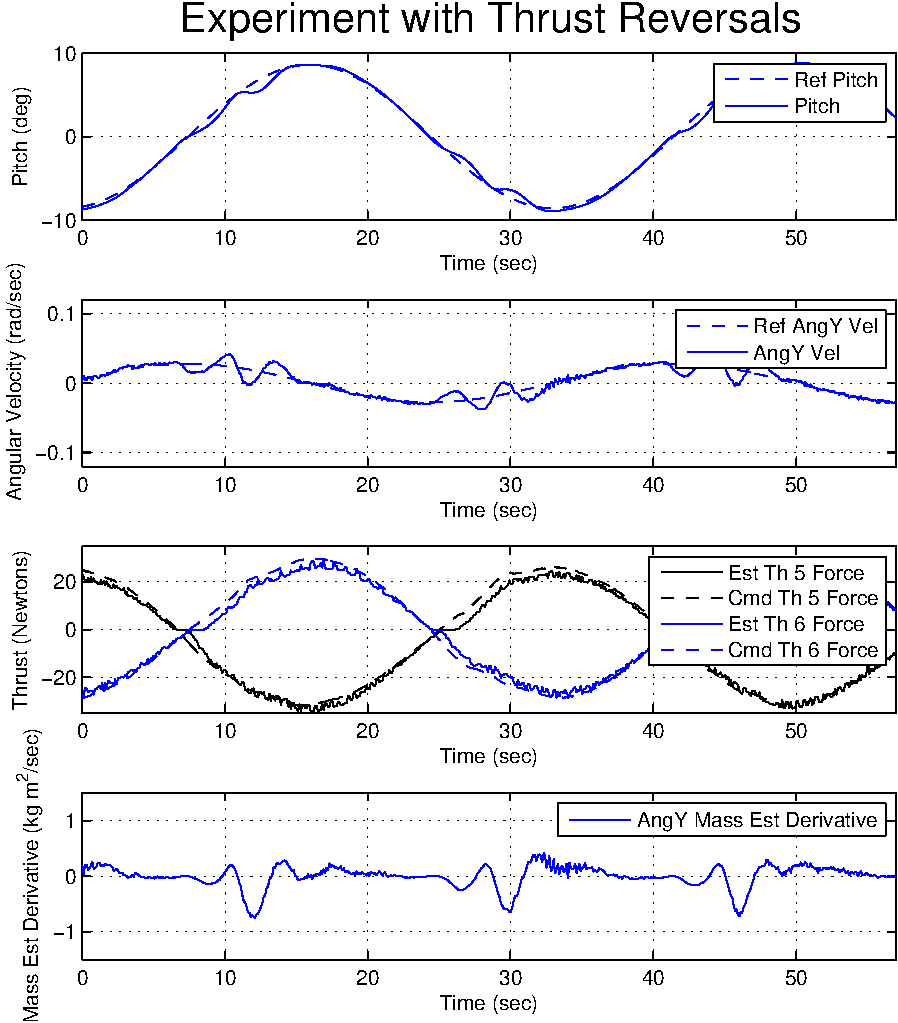
\includegraphics[width=150mm]{./chUV_AMBC/images/stictionErrorWithThrustReversals}
  \end{center}
  \caption{ 
%Data from two experiments where   For both
%    experiments an uncoupled model was assumed, initial parameter
%    estimates taken from the final values in Tables
%    \ref{chUV_AMBC.tb.quasistatic} and \ref{chUV_AMBC.tb.dynParam},
    Fifty five seconds of data from a experiment where \ac{AMBC} was used to
    follow a single \ac{DOF} reference trajectory in pitch.  Following
    the reference trajectory required thrust reversals. Thruster force
    was estimated using measured propeller angular velocity.  In the
    commanded/estimated thruster subplot, a short period of thruster
    stiction is seen at each thrust reversal.  The effects of thruster
    stiction are seen in both the pitch and angular velocity plots as
    deviations from each state's respective reference trajectory. In
    the pitch mass estimate derivative, the parameter update law is
    seen to have a large negative spike after each thrust reversal.}
  \label{chUV_AMBC.fig.stictionErrorWithThRev}
\end{figure*}
\end{center}

\begin{center}
\begin{figure*}[htbp]
  \begin{center}
    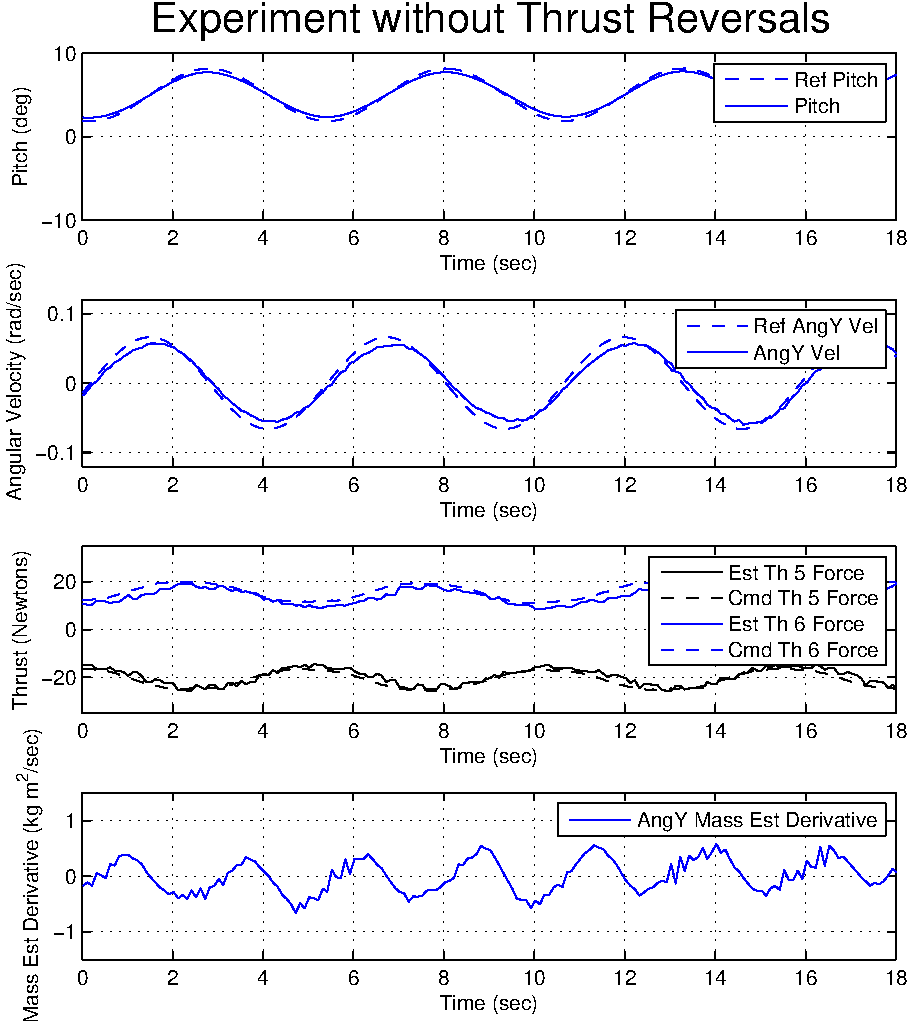
\includegraphics[width=150mm]{./chUV_AMBC/images/stictionErrorWoThrustReversals}
  \end{center}
  \caption{Eighteen seconds of data from a experiment where \ac{AMBC} was
    used to follow a single \ac{DOF} reference trajectory in pitch.
    Following the reference trajectory did not require thrust
    reversals. Thruster force was estimated using measured propeller
    angular velocity.  In the commanded/estimated thruster subplot
    thruster stiction is not observed.  The chain of events leading to a
    large negative spike in the pitch mass update law are not present
    in this experiment.}
  \label{chUV_AMBC.fig.stictionErrorWithoutThRev}
\end{figure*}
\end{center}

%experimental.tex
%\section{Experimental Evaluation}\label{sec.experimental}



\subsection{Experimental Evaluation of Two-Step Method}
\label{chUV_AMBC.sec.twoStepExp}

In this Section we report an experimental evaluation of the two-step
algorithm reported in Section \ref{chUV_AMBC.sec.twoStepMethod}.

The first step is identifying the gravitational and buoyancy
parameters for the \ac{UV} using the adaptive tracking controller for
plant model (\ref{chUV_AMBC.eq.plantQS}).  The reference trajectory
was constant in translational position and heading, with slow changes
in pitch and roll to provide quasi-static motion.  For this experiment
we used a sinusoidal pitch reference trajectory with a magnitude of
$0.2$ rad and frequency of $34$ Hz and a sinusoidal roll reference
trajectory with a magnitude of $0.15$ rad and frequency of $42$
Hz. The gains used were $k_p=300$, $k_d=100$,
$\gamma_{g}=\gamma_{b_1}=\gamma_{b_2}=0.5$, and $\gamma_{b_3}=10.0$.
Over a 90 minute experiment the gravitational and buoyancy parameters
were stable and converged to the physically realistic values shown in
Table \ref{chUV_AMBC.tb.quasistatic}.

\begin{table}[htbp]
\ssp
\caption{Gravitational Parameters Identified During Quasi-Static Motion}
\begin{center}
\begin{tabular}{c|cccc}
 & $g$ & $b_1$ & $b_2$ & $b_3$ \\
 & {\it N} & {\it N m} & {\it N m} & {\it N m} \\ \hline
Final & 3.59 & 1.696 & 3.09 & 300 \\
\end{tabular}
\end{center}
\label{chUV_AMBC.tb.quasistatic}
\vspace*{-5mm}
\end{table}


The second step uses the identified parameters from Table
\ref{chUV_AMBC.tb.quasistatic} in a \ac{AMBC} which estimates the
mass and drag parameters, as described in Section
\ref{chUV_AMBC.sec.twoStepMethod}.
%
In the second step of the two-step \ac{AMBC} algorithm the reference
trajectory specified was RefTraj1 from Table
\ref{chUV_AMBC.tb.expStat}; the mass and drag parameters were
initialized to zero; and the gains used were $k_p=300$, $k_d=1000$,
$\gamma_{m_i}=1000$, and $\gamma_{d_i}=5000$.  Over a four and a half
hour experiment all 12 mass and drag parameters were observed to be
stable and converge to physically realistic values.  Table
\ref{chUV_AMBC.tb.dynParam} records the initial and final states for
each dynamic parameter estimate.

\begin{table}[htbp]
\ssp
\caption{Parameters Identified with two-step \ac{AMBC} during 
  Dynamic Motion Trajectory-Tracking}
\begin{center}
\begin{tabular}{c|cccc}
 & $m_i(t_o)$ & $m_i(t_f)$ & $d_i(t_o)$ & $d_i(t_f)$ \\ \hline
Trans X \ac{DOF} & 0.0 {\it kg}& 628 {\it kg}& 0.0 {\it $\frac{\text{N}~\text{s}^2}{\text{m}^2}$}& -1259 {\it $\frac{\text{N}~\text{s}^2}{\text{m}^2}$}\\
Trans Y \ac{DOF} & 0.0 {\it kg}& 791 {\it kg}& 0.0 {\it $\frac{\text{N}~\text{s}^2}{\text{m}^2}$}& -1429 {\it $\frac{\text{N}~\text{s}^2}{\text{m}^2}$}\\
Trans Z \ac{DOF} & 0.0 {\it kg}&1043 {\it kg}& 0.0 {\it $\frac{\text{N}~\text{s}^2}{\text{m}^2}$}& -3083 {\it $\frac{\text{N}~\text{s}^2}{\text{m}^2}$}\\
Angular X \ac{DOF} & 0.0 {\it kg $\text{m}^2$}& 95.7 {\it kg $\text{m}^2$}& 0.0 {\it N $\text{s}^2$}& -727.1 {\it N $\text{s}^2$}\\
Angular Y \ac{DOF} & 0.0 {\it kg $\text{m}^2$}& 145.3 {\it kg $\text{m}^2$}& 0.0 {\it N $\text{s}^2$}& -783.4 {\it N $\text{s}^2$}\\
Angular Z \ac{DOF} & 0.0 {\it kg $\text{m}^2$}& 110.2 {\it kg $\text{m}^2$}& 0.0 {\it N $\text{s}^2$}& -465.6 {\it N $\text{s}^2$}\\
\end{tabular}
\end{center}
\label{chUV_AMBC.tb.dynParam}
\vspace*{-5mm}
\end{table}

\subsubsection{Two-Step \ac{AMBC} Trajectory Tracking Performance}

Figure \ref{chUV_AMBC.fig.MNE_All} compares the performance of the
second step of the two-step \ac{AMBC} to a \ac{PDC} with comparable
gains.  These two plots contain the exponential position and velocity
\ac{MNE} for the \ac{PDC} and two-step \ac{AMBC} experimental run.
Both controllers were following the reference trajectory RefTraj1 from
Table \ref{chUV_AMBC.tb.expStat} as well as using $k_p=300$ and
$k_d=100$.
%
The \ac{PDC} \acp{MNE} values were calculated using 10 minutes of
data.  
%
The two-step \ac{AMBC} \acp{MNE} values were calculated
for consecutive 15 minutes windows.
%
Note that after parameter convergence the two-step \ac{AMBC} provides
$30\%$ better position tracking and $8\%$ worse velocity tracking than
\ac{PDC} with similar gains.
%
% Thus two-step \ac{AMBC} Since position trajectory tracking is typically
% the goal of current \ac{UV} controllers, this controller provides
% significant advantages over standard \ac{PDC} control method for 6-\ac{DOF}
% motion.

Table \ref{chUV_AMBC.tb.trajTrackMAE} reports the trajectory tracking
\ac{MAE} values of individual \ac{DOF} for both the \ac{PDC} and
two-step \ac{AMBC} experiments.
%
The \ac{PDC} \acp{MAE} values were calculated using 10 minutes of
data.  
%
The two-step \ac{AMBC} \acp{MAE} values were calculated
for consecutive 15 minutes windows.
%
For each of the position \ac{DOF}, two-step \ac{AMBC} \ac{MAE} values
were smaller than \ac{PDC} values.
%
With the exception of heading, two-step \ac{AMBC} position trajectory
tracking improved in each \ac{DOF} as the parameter adaptation process
progressed.
%
Of the velocity \ac{DOF}, two-step \ac{AMBC} only outperformed
\ac{PDC} in the x and y angular velocity \ac{DOF}.
%
With the exception of y angular velocity, two-step \ac{AMBC} velocity
trajectory-tracking performance degraded slightly as the parameter
adaptation process occurred.
%
For the \ac{DOF} in which trajectory-tracking is not improving, this
could be an effect of unmodeled thruster dynamics or other dynamics
which are not included in the uncoupled lumped-parameter model of
\ac{UV} dynamics used in our \ac{AMBC} algorithm.
%
However, taken as a whole, this experimental evaluation indicates that
\ac{AMBC} can provide increased trajectory-tracking performance in the
presence of unmodeled thruster dynamics.




\begin{center}
\begin{figure}[htbp]
  \begin{center}
    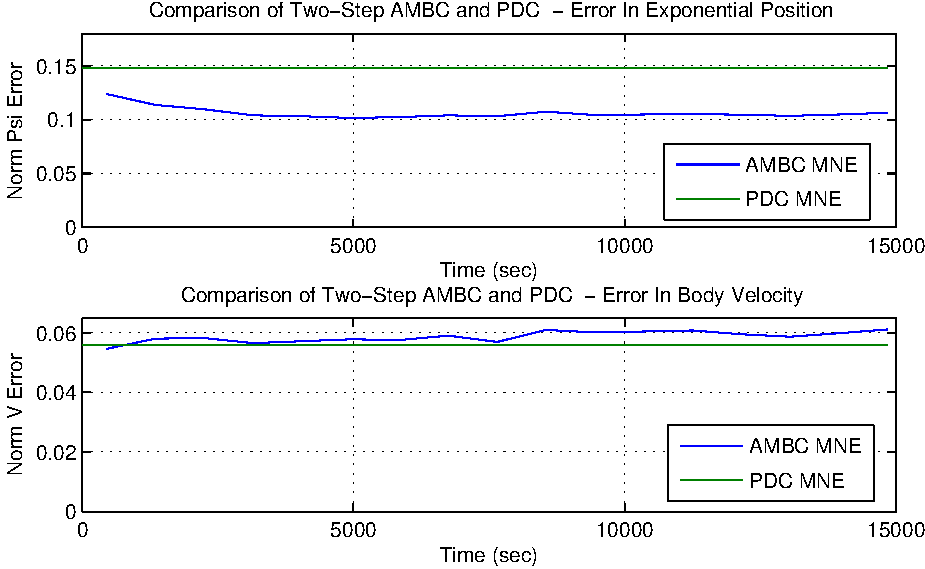
\includegraphics[width=150mm]{./chUV_AMBC/images/MNE_All}
  \end{center}
  \caption{ Exponential position and velocity \ac{MNE} values for the
    experimental evaluations of two controllers, \ac{PDC} and two-step
    \ac{AMBC}.  Both controllers were following the same reference
    trajectory (RefTraj1 from Table \ref{chUV_AMBC.tb.expStat}) as
    well as using the gains $k_p=300$ and $k_d=100$.  The \ac{PDC}
    \ac{MNE} values were calculated using 10 minutes of data, this
    single value is plotted in green across the entire figure.  The
    two-step \ac{AMBC} \ac{MNE} values were calculated for consecutive
    15 minute windows and plotted in blue. }
  \label{chUV_AMBC.fig.MNE_All}
\vspace*{-5mm}
\end{figure}
\end{center}

% \begin{sidewaystable*}
% \ssp
% \fontsize{8pt}{8pt}\selectfont
% \caption{Mean Absolute Error values over different pieces on time.}
% \begin{center}
% \begin{tabular}{c|ccccccccccccc} 
%     Parameter & Time  &&&&&&&&&&&& \\              
%           Set & Block & PosX & PosY & PosZ & Hea & Pit & Rol & BodVelX & BodVelY & BodVelZ & AngVelX & AngVelY & AngVelZ \\ \hline 
% \\
% \ac{PDC} Exp  &      ALL   & 0.076m & 0.061m & 0.058m & 0.028rad & 0.047rad & 0.04rad & 0.0172m/s & 0.021m/s & 0.0156m/s & 0.021rad/s & 0.028rad/s & 0.0078rad/s \\ \hline
% \\
% \ac{AMBC} Exp & 0-14 min & 0.059m & 0.051m & 0.064m & 0.021rad & 0.023rad & 0.0181rad & 0.022m/s & 0.023m/s & 0.0194m/s & 0.0136rad/s & 0.017rad/s & 0.0134rad/s \\
% \\
% \ac{AMBC} Exp & 0-14 min & 0.051m & 0.045m & 0.063m & 0.022rad & 0.0196rad & 0.0184rad & 0.024m/s & 0.023m/s & 0.02m/s & 0.0137rad/s & 0.0157rad/s & 0.0162rad/s \\
% \\
% \ac{AMBC} Exp & 15-29 min & 0.047m & 0.046m & 0.057m & 0.021rad & 0.0196rad & 0.0171rad & 0.023m/s & 0.025m/s & 0.02m/s & 0.013rad/s & 0.0169rad/s & 0.0153rad/s \\
% \\
% \ac{AMBC} Exp & 30-44 min & 0.046m & 0.045m & 0.054m & 0.0192rad & 0.018rad & 0.0165rad & 0.023m/s & 0.025m/s & 0.0196m/s & 0.0136rad/s & 0.0157rad/s & 0.0149rad/s \\
% \\
% \ac{AMBC} Exp & 45-59 min & 0.046m & 0.043m & 0.052m & 0.021rad & 0.0174rad & 0.0162rad & 0.024m/s & 0.025m/s & 0.019m/s & 0.0136rad/s & 0.0162rad/s & 0.0161rad/s \\
% \\
% \ac{AMBC} Exp & 60-74 min & 0.047m & 0.047m & 0.046m & 0.0198rad & 0.0174rad & 0.0156rad & 0.023m/s & 0.027m/s & 0.0179m/s & 0.0138rad/s & 0.0168rad/s & 0.0152rad/s \\
% \\
% \ac{AMBC} Exp & 75-89 min & 0.047m & 0.045m & 0.05m & 0.021rad & 0.0168rad & 0.0155rad & 0.024m/s & 0.024m/s & 0.0192m/s & 0.0143rad/s & 0.0164rad/s & 0.0155rad/s \\
% \\
% \ac{AMBC} Exp & 90-104 min & 0.046m & 0.046m & 0.052m & 0.022rad & 0.0174rad & 0.0155rad & 0.024m/s & 0.026m/s & 0.0198m/s & 0.014rad/s & 0.0165rad/s & 0.0162rad/s \\
% \\
% \ac{AMBC} Exp & 105-119 min & 0.048m & 0.044m & 0.05m & 0.022rad & 0.0162rad & 0.0153rad & 0.021m/s & 0.025m/s & 0.021m/s & 0.0133rad/s & 0.0159rad/s & 0.0151rad/s \\
% \\
% \ac{AMBC} Exp & 120-134 min & 0.049m & 0.048m & 0.054m & 0.021rad & 0.0182rad & 0.015rad & 0.023m/s & 0.027m/s & 0.023m/s & 0.0145rad/s & 0.0169rad/s & 0.016rad/s \\
% \\
% \ac{AMBC} Exp & 135-149 min & 0.049m & 0.045m & 0.05m & 0.022rad & 0.0177rad & 0.0145rad & 0.025m/s & 0.026m/s & 0.021m/s & 0.0145rad/s & 0.0172rad/s & 0.0165rad/s \\
% \\
% \ac{AMBC} Exp & 150-164 min & 0.05m & 0.046m & 0.049m & 0.021rad & 0.0166rad & 0.0155rad & 0.024m/s & 0.026m/s & 0.021m/s & 0.0143rad/s & 0.0161rad/s & 0.0167rad/s \\
% \\
% \ac{AMBC} Exp & 165-179 min & 0.049m & 0.046m & 0.052m & 0.021rad & 0.0168rad & 0.0151rad & 0.024m/s & 0.026m/s & 0.022m/s & 0.0145rad/s & 0.0167rad/s & 0.0153rad/s \\
% \\
% \ac{AMBC} Exp & 180-194 min & 0.048m & 0.047m & 0.05m & 0.021rad & 0.017rad & 0.0149rad & 0.024m/s & 0.024m/s & 0.021m/s & 0.0141rad/s & 0.0165rad/s & 0.016rad/s \\
% \\
% \ac{AMBC} Exp & 195-209 min & 0.05m & 0.045m & 0.049m & 0.022rad & 0.0169rad & 0.0149rad & 0.023m/s & 0.026m/s & 0.02m/s & 0.0139rad/s & 0.0163rad/s & 0.0161rad/s \\
% \\
% \ac{AMBC} Exp & 210-224 min & 0.05m & 0.046m & 0.049m & 0.021rad & 0.0174rad & 0.0147rad & 0.024m/s & 0.027m/s & 0.021m/s & 0.0142rad/s & 0.0166rad/s & 0.0148rad/s \\
% \\
% \ac{AMBC} Exp & 225-239 min & 0.047m & 0.046m & 0.054m & 0.022rad & 0.0172rad & 0.0147rad & 0.025m/s & 0.026m/s & 0.023m/s & 0.0145rad/s & 0.0164rad/s & 0.0169rad/s \\
% \end{tabular}
% \end{center}
% \label{chUV_AMBC.tb.MAE}
% \end{sidewaystable*}


\begin{sidewaystable*}
\ssp
\fontsize{10pt}{10pt}\selectfont
\caption{\acf{MAE} values for both the \ac{PDC} and two-step \ac{AMBC}
  experiments.  The \ac{MAE} for each \ac{DOF} is shown. 10 minutes of
  experimental data were used to calculate the \ac{PDC} \acp{MAE}.
  \ac{AMBC} \acp{MAE} were calculated for consecutive 15 minute
  windows spread over the 3 hour experiment.}
\begin{center}
\begin{tabular}{c|ccccccccccccc} 
    Parameter & Time  &&&&&&&&&&&& \\              
          Set & Block & PosX & PosY & PosZ & Hea & Pit & Rol & BodVelX & BodVelY & BodVelZ & AngVelX & AngVelY & AngVelZ \\  
      {\it -} & {\it min} & {\it m}   &  {\it m}  &  {\it m}  &{\it rad} &{\it rad} &{\it rad} &{\it m/sec} &{\it m/sec} &{\it m/sec} &{\it rad/sec} &{\it rad/sec} &{\it rad/sec} \\ \hline 
\\
\ac{PDC} Exp  &    -   & 0.076  & 0.061  & 0.058  & 0.028  & 0.047  & 0.04  & 0.0172  & 0.021  & 0.0156  & 0.021  & 0.028  & 0.0078  \\ \hline
\\
\ac{AMBC} Exp & 0-14   & 0.059  & 0.051  & 0.064  & 0.021  & 0.023  & 0.0181  & 0.022  & 0.023  & 0.0194  & 0.0136  & 0.017  & 0.0134  \\
\\
\ac{AMBC} Exp & 15-29   & 0.051  & 0.045  & 0.063  & 0.022  & 0.0196  & 0.0184  & 0.024  & 0.023  & 0.02  & 0.0137  & 0.0157  & 0.0162  \\
\\
\ac{AMBC} Exp & 30-44   & 0.047  & 0.046  & 0.057  & 0.021  & 0.0196  & 0.0171  & 0.023  & 0.025  & 0.02  & 0.013  & 0.0169  & 0.0153  \\
\\
\ac{AMBC} Exp & 45-59   & 0.046  & 0.045  & 0.054  & 0.0192  & 0.018  & 0.0165  & 0.023  & 0.025  & 0.0196  & 0.0136  & 0.0157  & 0.0149  \\
\\
\ac{AMBC} Exp & 60-74   & 0.046  & 0.043  & 0.052  & 0.021  & 0.0174  & 0.0162  & 0.024  & 0.025  & 0.019  & 0.0136  & 0.0162  & 0.0161  \\
\\
\ac{AMBC} Exp & 75-89   & 0.047  & 0.047  & 0.046  & 0.0198  & 0.0174  & 0.0156  & 0.023  & 0.027  & 0.0179  & 0.0138  & 0.0168  & 0.0152  \\
\\
\ac{AMBC} Exp & 90-104   & 0.047  & 0.045  & 0.05  & 0.021  & 0.0168  & 0.0155  & 0.024  & 0.024  & 0.0192  & 0.0143  & 0.0164  & 0.0155  \\
\\
\ac{AMBC} Exp & 105-119   & 0.046  & 0.046  & 0.052  & 0.022  & 0.0174  & 0.0155  & 0.024  & 0.026  & 0.0198  & 0.014  & 0.0165  & 0.0162  \\
\\
\ac{AMBC} Exp & 120-134  & 0.048  & 0.044  & 0.05  & 0.022  & 0.0162  & 0.0153  & 0.021  & 0.025  & 0.021  & 0.0133  & 0.0159  & 0.0151  \\
\\
\ac{AMBC} Exp & 135-149   & 0.049  & 0.048  & 0.054  & 0.021  & 0.0182  & 0.015  & 0.023  & 0.027  & 0.023  & 0.0145  & 0.0169  & 0.016  \\
\\
\ac{AMBC} Exp & 150-164   & 0.049  & 0.045  & 0.05  & 0.022  & 0.0177  & 0.0145  & 0.025  & 0.026  & 0.021  & 0.0145  & 0.0172  & 0.0165  \\
\\
\ac{AMBC} Exp & 165-179   & 0.05  & 0.046  & 0.049  & 0.021  & 0.0166  & 0.0155  & 0.024  & 0.026  & 0.021  & 0.0143  & 0.0161  & 0.0167  \\
\\
\ac{AMBC} Exp & 180-194   & 0.049  & 0.046  & 0.052  & 0.021  & 0.0168  & 0.0151  & 0.024  & 0.026  & 0.022  & 0.0145  & 0.0167  & 0.0153  \\
\\
\ac{AMBC} Exp & 195-209   & 0.048  & 0.047  & 0.05  & 0.021  & 0.017  & 0.0149  & 0.024  & 0.024  & 0.021  & 0.0141  & 0.0165  & 0.016  \\
\\
\ac{AMBC} Exp & 210-224   & 0.05  & 0.045  & 0.049  & 0.022  & 0.0169  & 0.0149  & 0.023  & 0.026  & 0.02  & 0.0139  & 0.0163  & 0.0161  \\
\\
\ac{AMBC} Exp & 225-239   & 0.05  & 0.046  & 0.049  & 0.021  & 0.0174  & 0.0147  & 0.024  & 0.027  & 0.021  & 0.0142  & 0.0166  & 0.0148  \\
\\
\ac{AMBC} Exp & 240-255   & 0.047  & 0.046  & 0.054  & 0.022  & 0.0172  & 0.0147  & 0.025  & 0.026  & 0.023  & 0.0145  & 0.0164  & 0.0169  \\
\end{tabular}
\end{center}
\label{chUV_AMBC.tb.trajTrackMAE}
\end{sidewaystable*}


\subsubsection{Two-Step \ac{AMBC} Parameter Cross-Validation}

In addition to providing trajectory-tracking, \ac{AMBC} has also been
proposed to identify \ac{UV} models.
%
Two questions arise: 
%
\begin{itemize}
\item ``How good is the identified model at reproducing vehicle performance?''
%``When considering the time series of parameter
%estimations, will the capacity of the models which used these
%parameter estimations get better at matching vehicle performance as
%time increases?''
%
\item``Considering the time series of parameter estimates, do the
  resulting plant models get better at matching \ac{JHUROV}
  performance as the parameter adaptation process progresses?''
\end{itemize}
%

To address these questions we preformed a cross-validation experiment
(Appendix \ref{appenJHUHTF.sec.paramEvalMethod}) by driving the
\ac{JHUROV} to follow RefTraj2 from Table \ref{chUV_AMBC.tb.expStat}.
%the \ac{UV} states and thrust inputs were recorded for 10 minutes.
%
\Cref{chUV_AMBC.fig.posOLO,chUV_AMBC.fig.angVelOLO,chUV_AMBC.fig.bodVelOLO}
show the ability of the identified model to match vehicle performance
in forward simulation increases during parameter adaptation.
%
Each Figure shows experimentally measured states verses the states
from numerical simulations; each numerical simulation uses a model
identified by the two-step \ac{AMBC} after a set amount of time.
%
Each \ac{JHUROV} simulation used the thrust inputs recorded and
initial \ac{JHUROV} states to create a forward
simulation. % of vehicle performance.
%
All eight open-loop-stable states are plotted.
%
In both the plots and listed \ac{MAE} values, the capacity of the
identified parameters to model vehicle performance in every \ac{DOF}
increases as time progresses.
%
The fact that the parameter estimates are progressively improving
suggests that the parameter adaptation process is working despite the
presence of unmodeled thruster dynamics.



As was seen with \ac{AID} and \ac{LS} in Sections
\ref{chUV_AID.sec.UVSO3exp} and \ref{chUV_AID.sec.UVSE3exp}, the
models identified using two-step \ac{AMBC} were not able to reproduce
the highest frequency fluctuation's observed experimentally (such as
those seen in the x angular velocity subplots of Figure
\ref{chUV_AMBC.fig.angVelOLO}).
%
However, the states shown from simulating a model using the ``5000
sec'' parameter set (the final parameter set included in this
analysis) indicate that \ac{AMBC} can produce parameter estimates
which result in accurate plant models.




\begin{center}
\begin{figure}[htbp]
  \begin{center}
    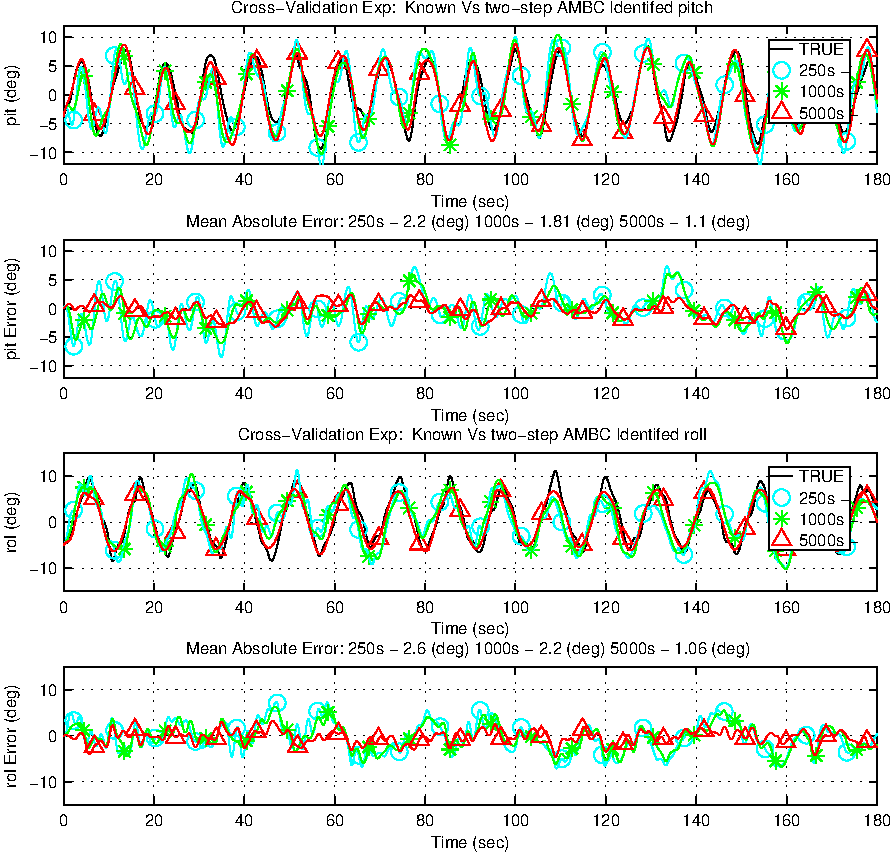
\includegraphics[width=150mm]{./chUV_AMBC/images/OLO_angPos}
  \end{center}
  \caption{ Representative data of experimental and simulated
    \ac{JHUROV} states during 6-\ac{DOF} dynamic operation.  In the
    roll and pitch plots the measured state is plotted together with
    the position estimates from three \ac{JHUROV} simulations. The
    three parameter sets were taken from the time history of parameter
    adaptation recorded during the two-step \ac{AMBC} experiment.  The
    '250s' forward simulation (plotted in blue and marked with
    circles) models \ac{JHUROV} performance using parameters
    identified after 250 seconds of parameter adaptation.  Similarly
    the '1000s' forward simulation (plotted in green and marked with
    stars) and '5000s' forward simulation (plotted in red and marked
    with triangles) use parameters identified after 1000 and 5000
    seconds of parameter adaptation respectively.  For each \ac{DOF},
    the error between the measured positions and their estimates is
    shown.  }
  \label{chUV_AMBC.fig.posOLO}
\end{figure}
\end{center}

\begin{center}
\begin{figure}[htbp]
  \begin{center}
    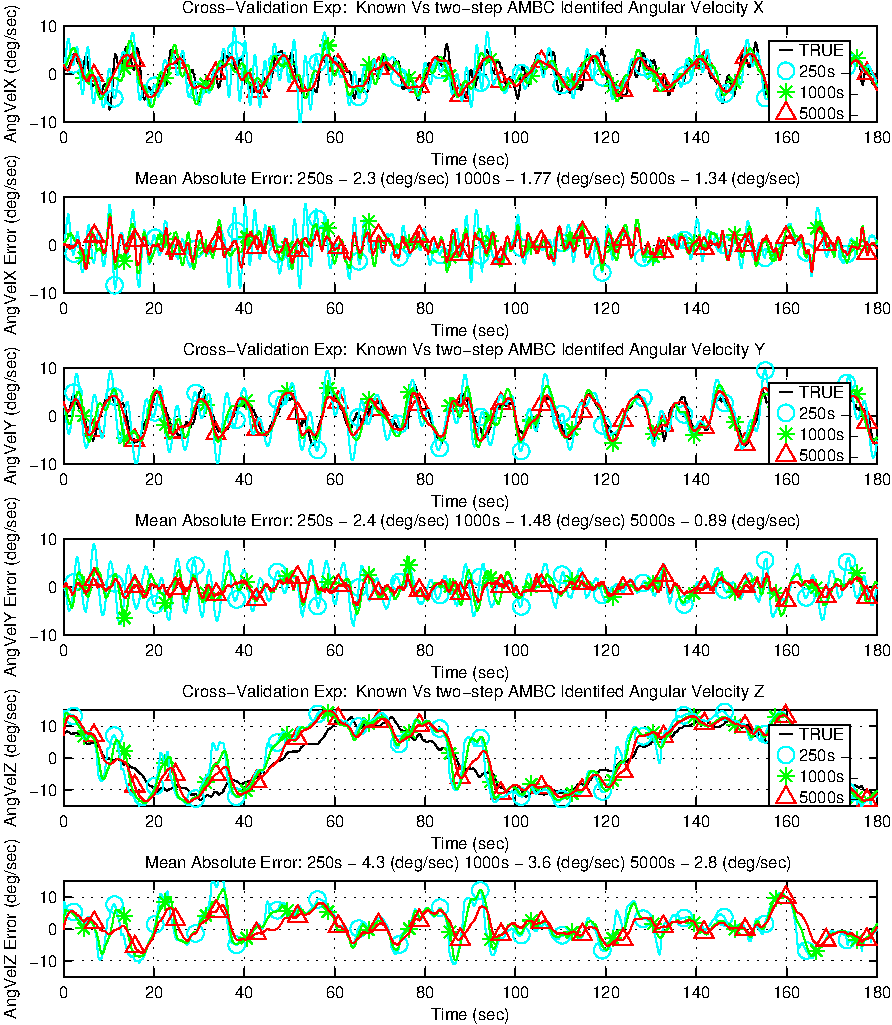
\includegraphics[width=150mm]{./chUV_AMBC/images/OLO_angVel}
  \end{center}
  \caption{ Representative data of experimental and simulated
    \ac{JHUROV} states during 6-\ac{DOF} dynamic operation.  In the
    three angular velocity plots, the measured state is plotted
    together with the velocity estimates from three \ac{JHUROV}
    simulations. The three parameter sets were taken from the time
    history of parameter adaptation recorded during the two-step
    \ac{AMBC} experiment.  See Figure \ref{chUV_AMBC.fig.posOLO}
    caption for further information on each parameter set.  For each
    \ac{DOF}, the error between the measured positions and their
    estimates is shown.  }
  \label{chUV_AMBC.fig.angVelOLO}
\end{figure}
\end{center}

\begin{center}
\begin{figure}[htbp]
  \begin{center}
    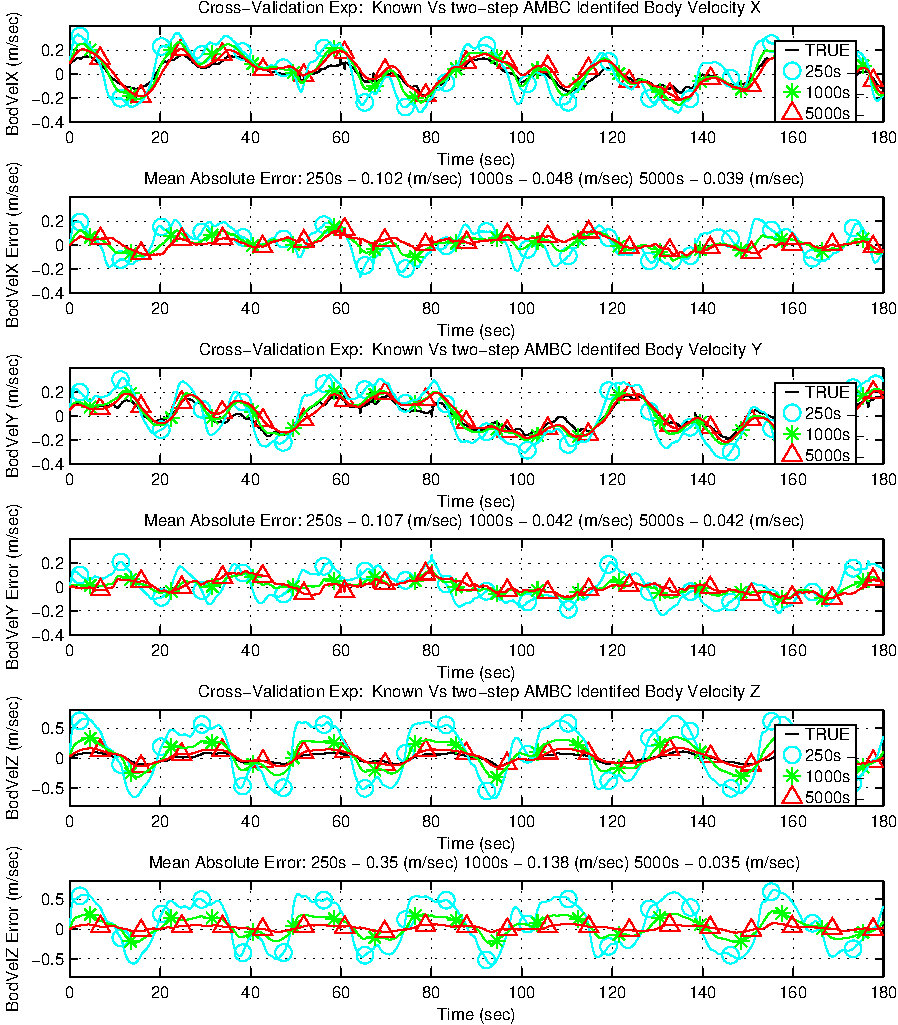
\includegraphics[width=150mm]{./chUV_AMBC/images/OLO_bodyVel}
  \end{center}
  \caption{ Representative data of experimental and simulated
    \ac{JHUROV} states during 6-\ac{DOF} dynamic operation.  In the
    three body velocity plots, the measured state is plotted together
    with the velocity estimates from three \ac{JHUROV}
    simulations. The three parameter sets were taken from the time
    history of parameter adaptation recorded during the two-step
    \ac{AMBC} experiment.  See Figure \ref{chUV_AMBC.fig.posOLO}
    caption for further information on each parameter set.  For each
    \ac{DOF}, the error between the measured positions and their
    estimates is shown.  }
  \label{chUV_AMBC.fig.bodVelOLO}
\end{figure}
\end{center}
 


\subsection{The Effects of Unmodeled Thruster Dynamics on \ac{AMBC}}

The experiment reported in Section
\ref{chUV_AMBC.sec.fullAnalysisFailure} shows, curiously, a clear
differentiation in parameter adaptation performance; unstable
parameter adaption occurred only in the parameter estimates associated
with pitch and roll dynamics.
%
To further explore this effect, in Section
\ref{chUV_AMBC.sec.singleDOFAnalysisFailure} we investigated parameter
adaptation during pitch-only reference trajectory excitation.
%
These data show thrust reversals cause parameter instability.
%
Further, the thruster angular velocity data indicate a difference
between the actual and commanded torques applied to the vehicle. 
%
Based on our knowledge of the \ac{JHUROV} control system and thruster
design, the data from these pitch-only experiments suggest that
unmodeled thruster dynamics are present during thrust reversals.
%
Without further experimental analysis we can not specify if the
specific mechanism causing unstable parameter adaptation is unmodeled
thruster mechanical dynamics, fluid dynamics, mechanical friction
during thrust reversals, or some combination of these mechanisms.
%
Regardless of the underlying source of modeling error, these
experiments suggest that unstable parameter adaptation will occur in
parameters associated with a given \ac{DOF} if the following three
conditions are met:
%
\begin{itemize}
\item mass and gravitational parameter estimates are adapting, 
\item there exists of a single attractive stability point for that \ac{DOF}, and
\item unmodeled thruster dynamics are present.
\end{itemize}


The success of two-step parameter adaptation supports this hypothesis.
%
Implementing the parameter estimation process in two steps removed
the need for simultaneous adaptation of the mass and buoyancy terms.
%
By separating parameter adaptation in this way, an ambiguity in the
adaptation process was removed.
%
Note the three factors listed imply that both the buoyancy and
mass parameter estimates will be affected in the same way by unmodeled
thruster dynamics during thrust reversals.  
%
From the perspective of the \ac{AMBC} algorithm, the deviations from
the position and velocity reference trajectories caused by unmodeled
thruster dynamics are indistinguishable from the deviations which
would occur if either of these parameter estimates (the buoyancy
torque estimate or the inertia estimate) were too large.
%
The effects of the inertia tensor and buoyancy torque parameters on
vehicle position and velocity are also coupled.
%
For instance there will be similarities between the dynamics of a
\ac{UV} with a large mass and large buoyancy torque and a \ac{UV} with
a small mass and small buoyancy torque for a proper scaling of these
properties.
%
During each period of unmodeled thruster dynamics, the simultaneous
unstable adaptation of the inertia and buoyancy estimates was
difficult for the \ac{AMBC} algorithm to overcome because the estimate
of vehicle dynamics was only slightly degraded by the physically
unrealistic changes in these parameter estimates.
%
Setting the buoyancy torque estimate to a fixed value during dynamic
maneuvers removes the possibility of simultaneous adaptation to
physically unrealistic values.






%  might still be close to values which are
% still good at approximating vehicle dynamics.
% %
% However, the difference tween
 
% adapt twoards physically unrealistic parameter values togeather, the
% difference in vehicle dynamnics

% Although these parameters play structrually
% different roles in UV dynamics their effects on the

% their effects for small angles are coupled,  that much
% of the UV modeling errors both having physically unrealstic values can


%  a different form when entering
% into the dynamics equation



%  or the if the
% estimated pitch inertia were too large both parameter update laws will
% experience a large negitive spike since the pitch or roll state
% lingering near zero

% Although   
